\subsection{Scaling of hairpin (un)zipping time}

The characteristic time of the unwinding process of double stranded DNA in function of the polymer length has been predicted numerous times with numerous simulation techniques. While most models indirectly take into account the helical structure of dsDNA, few models actually simulate the real physical structure. The topological structure of dsDNA however has a significant effect on the time scaling laws describing the mechanical zipping or unzipping \cite{carlon2010unwinding}.

We will look at the time scaling laws governing the formation and deformation of hairpin structures in ssDNA, where a single strand has complementary base pairs at both ends of the strand separated by a region (of a certain length $T_n$, eventually forming the loop of the hairpin) of non-complementary base pairs. In Figure \ref{results_hairpin} the formation of such a hairpin is simulated, using as strand configuration the sequence 5'-GCCTATTTTTTAATAGGC-3'. 

Baiesi, Barkema, Carlon \& Panja \cite{carlon2010unwinding} used Monte Carlo methods to determine that the time needed to unwind a double stranded polymer of length $N$ in a wound structure (yielding a basic simulation of the global dynamics of the unwinding process) scales like
\begin{equation}
\tau \sim N^{2.57\pm 0.03}.
\end{equation}

An older simulation by Baiesi \& Livi \cite{baiesi2009multiple} extends the scheme developed by Poland \& Scherega (PS) \cite{poland1966phase} to also incorporate topological structures such as the helicity winding of double stranded DNA, yielding unzipping behavior of
\begin{equation}
\tau \sim N^{3.0\pm 0.1}.
\end{equation}

For Monte Carlo zipping dynamics in a lattice DNA structure, Ferrantini \& Carlon \cite{carlon2011anomalous} found that the timescale needed for zipping two polymer strands scales anomalously as
\begin{equation}
\tau \sim N^{1.37\pm0.02}
\end{equation}
when quenching the polymers from a high temperature equilibrium configuration to a low temperature state. The unzipping when the strand is brought to a high temperature remained non-anomalous, scaling as $\tau \sim N$. The same model produces characteristic timescales that scale as $\tau \sim N^{2.26 \pm 0.02}$ when the strand is held at the critical temperature.

Simulations are performed on ssDNA sequences of the form (A)$_N$(T)$_N$ in an environment with $[\text{Na}^+] = 200$\,mM.
We opted to leave out an `inert' loop (for instance a sequence of C's in the middle) as to not slow the simulation down and delay the hairpin formation\footnote{We did not have sufficient time to measure the influence of loops and lengths thereof in hairpins, as most of our time was spent writing, debugging and verifying the implementation.
However, now that that part is finished, it is very straightforward to perform these simulations. The only necessity is sufficient CPU time.}.
It should also be noted that we used the base pairing coupling of the original Knotts model \cite{knotts2007coarse}, where $\epsAT = 2.77$\,kcal/mol and $\epsGC = 4.16$\,kcal/mol, instead of the one given in table \ref{couplingConstants}.
Due to time constraints, we could not compare the effect of this changed interaction strength (nor of different quenching temperatures) on the asymptotic scaling behaviour, but it is highly unlikely that it makes a significant contribution, due to the universality of such scaling laws.




In our simulations, at the start of every measurement run, the world is initialized with the chosen sequence built according to the B isoform as explained in section \ref{secStructure}.
The temperature is set to 20{\degree}C and the time it takes to reach a stable hairpin is measured, starting from the initial model B helix structure.
A hairpin is considered stable if it has at least $N-2$ bonded base pairs for a duration of minimally one nanosecond.

When the zipping criterion is reached, the hairpin is equilibrated for an additional 10 nanoseconds before setting the temperature to 180{\degree}C and starting the unzipping measurement.
This (very) high temperature was chosen to speed up the unzipping process.
The clock is stopped when the hairpin reaches a stable melted state, defined as having at most 2 bound base pairs for a duration of at least 1 nanosecond.

Simulations were run on hairpins with stem lengths between 10 and 100 monomers. At least 8 individual runs were generated per stem length, with the exception of $N = 60$ and $N = 80$, where we could only run 4 runs each due to time restrictions.

The results are show in Figure \ref{hairpinScaling}. We obtain the relations $\tauzip \sim N^\betazip$ and $\tauunzip \sim N^\betaunzip$ where $\betazip = 1.26 \pm 0.14$ and $\betaunzip = 2.62 \pm 0.09$

Note that the data shows large deviation from the fit for small $N$. This is to be expected, as uniform scaling behaviour only manifests itself in the limit of $N \to \infty$.


\begin{figure}[hbt]
\begin{center}
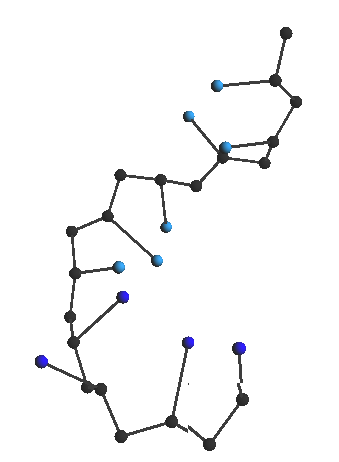
\includegraphics[width=4cm]{images/results_hairpin1}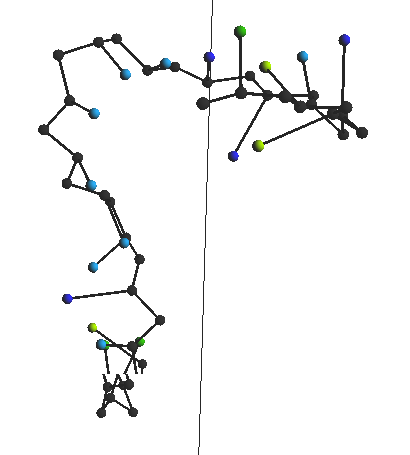
\includegraphics[width=5cm]{images/results_hairpin2}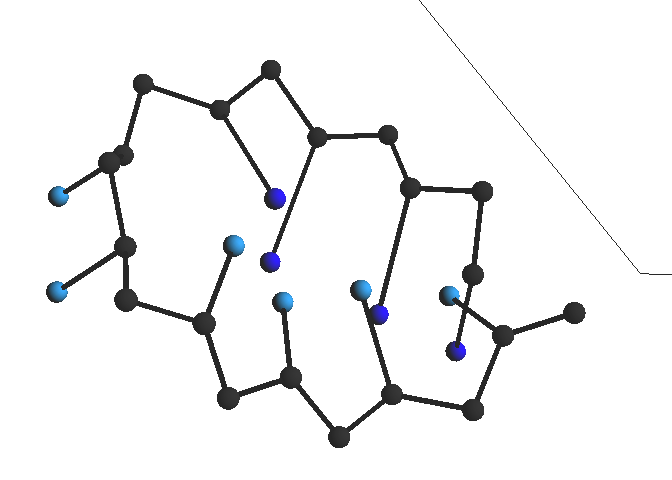
\includegraphics[width=5cm]{images/results_hairpin3}
\end{center}
\caption{Example of hairpin formation of a single strand with a stemlength of 4 base pairs and a loopsize of 2 monomers (5'-AAAATTTTTT-3'). This hairpin was formed after $\sim$ 20ns simulation time at 290K and salt concentration 100 mM.}
\label{results_hairpin}
\end{figure}


\subsection{Scaling of hairpin (un)zipping time}

The characteristic time of the unwinding process of double stranded DNA in function of the polymer length has been predicted numerous times with a multitude of simulation techniques. Most simple models ignore the helical structure of dsDNA, or only deal with it explicitly \cite{carlon2011anomalous, walter2011fractional}. A few models actually do explicitly take this helicity into account \cite{baiesi2009multiple, carlon2010unwinding}. Those last models showed that this helical structure has a significant effect on the time scaling laws describing the mechanical zipping or unzipping, leading to anomalous scaling exponents\cite{carlon2010unwinding}.


For Monte Carlo zipping dynamics in a lattice DNA structure, Ferrantini \& Carlon \cite{carlon2011anomalous} found that, ignoring helicit, the timescale needed for zipping two polymer strands scales anomalously as
\begin{equation}
\tau \sim N^{1.37\pm0.02}
\end{equation}
when quenching the polymers from a high temperature equilibrium configuration to a low temperature state. The unzipping when the strand is brought to a high temperature remained non-anomalous, scaling as $\tau \sim N$. The same model produces characteristic timescales that scale as $\tau \sim N^{2.26 \pm 0.02}$ when the strand is held at the critical temperature.

Baiesi, Barkema, Carlon \& Panja \cite{carlon2010unwinding} used Monte Carlo methods to determine the time needed to unwind a double stranded polymer of length $N$ in a wound structure, thus explicitly taking into account helicity. They found the result
\begin{equation}
\tau \sim N^{2.57\pm 0.03}.
\end{equation}

An older simulation by Baiesi \& Livi \cite{baiesi2009multiple} extends the scheme developed by Poland \& Scherega (PS) \cite{poland1966phase} to also incorporate topological structures such as the helicity winding of double stranded DNA, yielding unzipping behavior of
\begin{equation}
\tau \sim N^{3.0\pm 0.1}.
\end{equation}



We now use 3SPN model to explicitly find the scaling laws of hairpin formation for this more realistic model for DNA.
Simulations are performed on ssDNA sequences of the form (C)$_N$(G)$_N$ in an environment with $[\text{Na}^+] = 200$\,mM. A visualisation of hairpin formation for a short strand with $N = 15$ is shown in Figure \ref{results_hairpin}.

We opted to leave out an `inert' loop (for instance a sequence of C's in the middle) in the base sequence as to not slow the simulation down and delay the hairpin formation\footnote{We did not have sufficient time to measure the influence of loops and lengths thereof in hairpins, as most of our time was spent writing, debugging and verifying the implementation.
However, now that that part is finished, it is very straightforward to perform these simulations. The only necessity is sufficient CPU time.}.
It should also be noted that we used the base pairing coupling of the original Knotts model \cite{knotts2007coarse}, where $\epsAT = 2.77$\,kcal/mol and $\epsGC = 4.16$\,kcal/mol, instead of the one given in table \ref{couplingConstants}.
Due to time constraints, we could not compare the effect of this changed interaction strength (nor of different quenching temperatures) on the asymptotic scaling behaviour, but it is highly unlikely that it makes a significant contribution, due to the universality of such scaling laws.



In our simulations, at the start of every measurement run, the world is initialized with the chosen sequence built according to the B isoform as explained in section \ref{secStructure}.
The temperature is set to 20{\degree}C and the time it takes to reach a stable hairpin is measured, starting from the initial model B helix structure.
A hairpin is considered stable if it has at least $N-2$ bonded base pairs for a duration of minimally one nanosecond.

When the zipping criterion is reached, the hairpin is equilibrated for an additional 10 nanoseconds before setting the temperature to 180{\degree}C and starting the unzipping measurement.
This (very) high temperature was chosen to speed up the unzipping process.
The clock is stopped when the hairpin reaches a stable melted state, defined as having at most 2 bound base pairs for a duration of at least 1 nanosecond.

Simulations were run on hairpins with stem lengths between 10 and 100 monomers. At least 8 individual runs were generated per stem length, with the exception of $N = 60$ and $N = 80$, where we could only generate 4 runs each due to time restrictions, and $N = 100$ where we could only simulate 2 runs.

The results are show in Figure \ref{hairpinScaling}. We obtain the relations $\tauzip \sim N^\betazip$ and $\tauunzip \sim N^\betaunzip$ where $\betazip = 
1.26 \pm 0.14$ and $\betaunzip = 2.62 \pm 0.09$. We will further comment on these results in the next section.

Note that the data shows large deviation from the fit for small $N$ (The first two data points are not used for the fit). Some deviation is to be expected, as uniform scaling behaviour only manifests itself in the limit of $N \to \infty$. The geometry of the coarse grained model seems to suppress the formation of short hairpins, but note that the modelling such short hairpins (without an `inert loop') is not very physically relevant anyway, as in reality there will be no base pairings between the adjacent monomers in the middle of the hairpin strand.


\begin{figure}[hbt]
\begin{center}
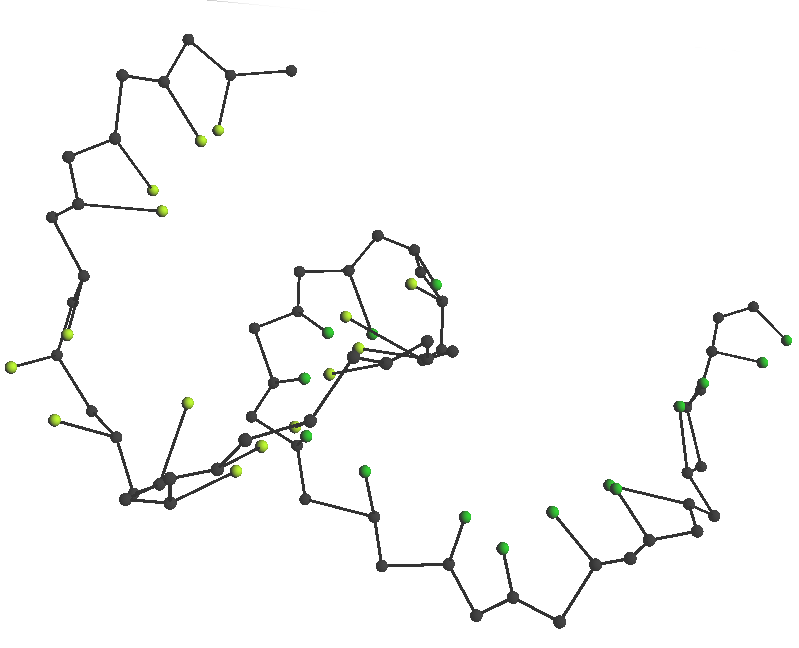
\includegraphics[width=4cm]{images/G15C15_1}
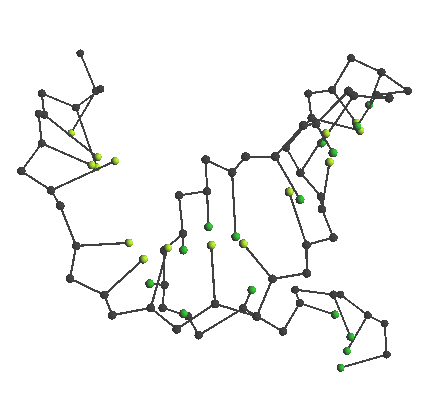
\includegraphics[width=4cm]{images/G15C15_2}
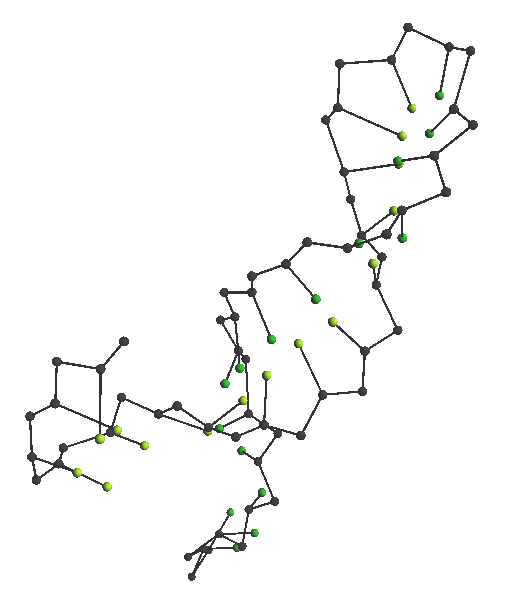
\includegraphics[width=4cm]{images/G15C15_3}
\end{center}
\caption{Visualisation of various stages of hairpin formation in a single strand of C$_{15}$G$_{15}$. In this case, the formation started at the center and zipped outwards.}
\label{results_hairpin}
\end{figure}


\subsection{Scaling of hairpin (un)zipping time}

The characteristic time of the unwinding process of double stranded DNA in function of the polymer length has been predicted numerous times with a multitude of simulation techniques. Most simple models ignore the helical structure of dsDNA, or only deal with it explicitly \cite{carlon2011anomalous, walter2011fractional}. A few models actually do explicitly take this helicity into account \cite{baiesi2009multiple, carlon2010unwinding}. Those last models showed that this helical structure has a significant effect on the time scaling laws describing the mechanical zipping or unzipping, leading to anomalous scaling exponents\cite{carlon2010unwinding}.


For Monte Carlo zipping dynamics in a lattice DNA structure, Ferrantini \& Carlon \cite{carlon2011anomalous} found that, ignoring helicit, the timescale needed for zipping two polymer strands scales anomalously as
\begin{equation}
\tau \sim N^{1.37\pm0.02}
\end{equation}
when quenching the polymers from a high temperature equilibrium configuration to a low temperature state. The unzipping when the strand is brought to a high temperature remained non-anomalous, scaling as $\tau \sim N$. The same model produces characteristic timescales that scale as $\tau \sim N^{2.26 \pm 0.02}$ when the strand is held at the critical temperature.

Baiesi, Barkema, Carlon \& Panja \cite{carlon2010unwinding} used Monte Carlo methods to determine the time needed to unwind a double stranded polymer of length $N$ in a wound structure, thus explicitly taking into account helicity. They found the result
\begin{equation}
\tau \sim N^{2.57\pm 0.03}.
\end{equation}

An older simulation by Baiesi \& Livi \cite{baiesi2009multiple} extends the scheme developed by Poland \& Scherega (PS) \cite{poland1966phase} to also incorporate topological structures such as the helicity winding of double stranded DNA, yielding unzipping behavior of
\begin{equation}
\tau \sim N^{3.0\pm 0.1}.
\end{equation}



We now use 3SPN model to explicitly find the scaling laws of hairpin formation for this more realistic model for DNA.
Simulations are performed on ssDNA sequences of the form (C)$_N$(G)$_N$ in an environment with $[\text{Na}^+] = 200$\,mM. A visualisation of hairpin formation for a short strand with $N = 15$ is shown in Figure \ref{results_hairpin}.

We opted to leave out an `inert' loop (for instance a sequence of C's in the middle) in the base sequence as to not slow the simulation down and delay the hairpin formation\footnote{We did not have sufficient time to measure the influence of loops and lengths thereof in hairpins, as most of our time was spent writing, debugging and verifying the implementation.
However, now that that part is finished, it is very straightforward to perform these simulations. The only necessity is sufficient CPU time.}.
It should also be noted that we used the base pairing coupling of the original Knotts model \cite{knotts2007coarse}, where $\epsAT = 2.77$\,kcal/mol and $\epsGC = 4.16$\,kcal/mol, instead of the one given in table \ref{couplingConstants}.
Due to time constraints, we could not compare the effect of this changed interaction strength (nor of different quenching temperatures) on the asymptotic scaling behaviour, but it is highly unlikely that it makes a significant contribution, due to the universality of such scaling laws.



In our simulations, at the start of every measurement run, the world is initialized with the chosen sequence built according to the B isoform as explained in section \ref{secStructure}.
The temperature is set to 20{\degree}C and the time it takes to reach a stable hairpin is measured, starting from the initial model B helix structure.
A hairpin is considered stable if it has at least $N-2$ bonded base pairs for a duration of minimally one nanosecond.

When the zipping criterion is reached, the hairpin is equilibrated for an additional 10 nanoseconds before setting the temperature to 180{\degree}C and starting the unzipping measurement.
This (very) high temperature was chosen to speed up the unzipping process.
The clock is stopped when the hairpin reaches a stable melted state, defined as having at most 2 bound base pairs for a duration of at least 1 nanosecond.

Simulations were run on hairpins with stem lengths between 10 and 100 monomers. At least 8 individual runs were generated per stem length, with the exception of $N = 60$ and $N = 80$, where we could only generate 4 runs each due to time restrictions, and $N = 100$ where we could only simulate 2 runs.

The results are show in Figure \ref{hairpinScaling}. We obtain the relations $\tauzip \sim N^\betazip$ and $\tauunzip \sim N^\betaunzip$ where $\betazip = 
1.26 \pm 0.14$ and $\betaunzip = 2.62 \pm 0.09$. We will further comment on these results in the next section.

Note that the data shows large deviation from the fit for small $N$ (The first two data points are not used for the fit). Some deviation is to be expected, as uniform scaling behaviour only manifests itself in the limit of $N \to \infty$. The geometry of the coarse grained model seems to suppress the formation of short hairpins, but note that the modelling such short hairpins (without an `inert loop') is not very physically relevant anyway, as in reality there will be no base pairings between the adjacent monomers in the middle of the hairpin strand.


\begin{figure}[hbt]
\begin{center}
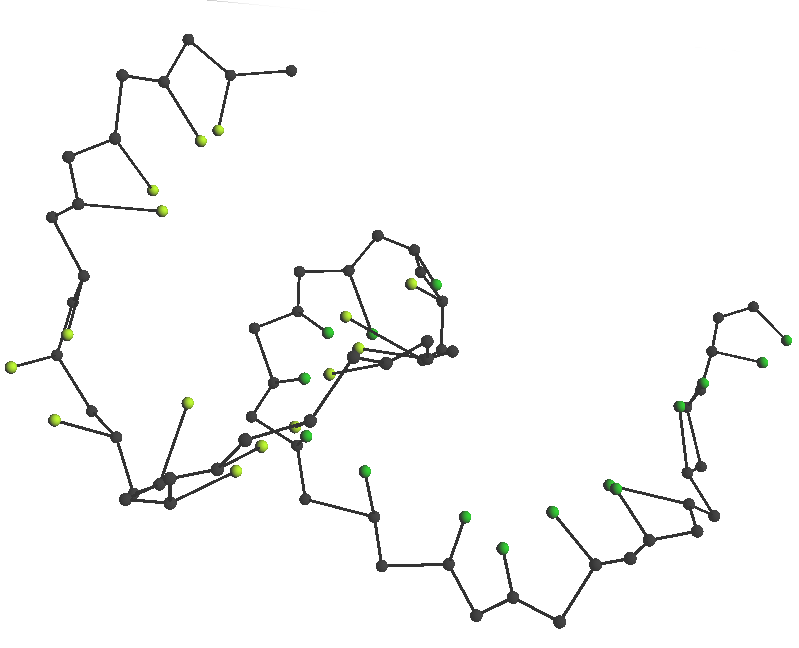
\includegraphics[width=4cm]{images/G15C15_1}
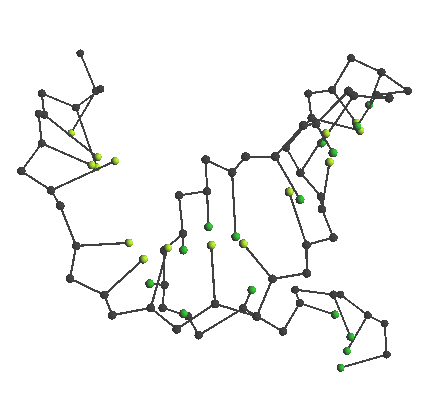
\includegraphics[width=4cm]{images/G15C15_2}
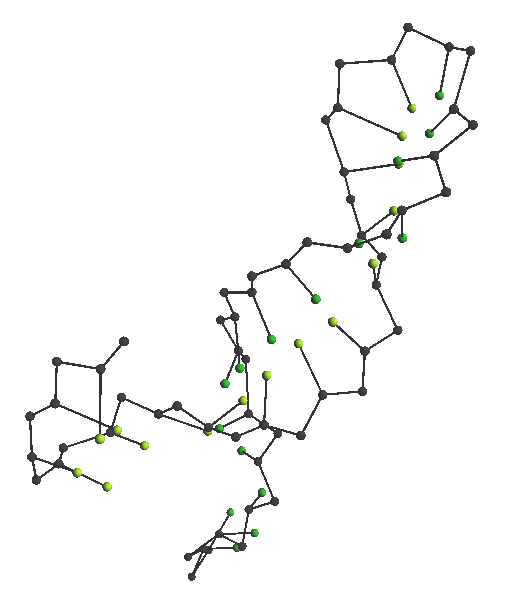
\includegraphics[width=4cm]{images/G15C15_3}
\end{center}
\caption{Visualisation of various stages of hairpin formation in a single strand of C$_{15}$G$_{15}$. In this case, the formation started at the center and zipped outwards.}
\label{results_hairpin}
\end{figure}


\subsection{Scaling of hairpin (un)zipping time}

The characteristic time of the unwinding process of double stranded DNA in function of the polymer length has been predicted numerous times with a multitude of simulation techniques. Most simple models ignore the helical structure of dsDNA, or only deal with it explicitly \cite{carlon2011anomalous, walter2011fractional}. A few models actually do explicitly take this helicity into account \cite{baiesi2009multiple, carlon2010unwinding}. Those last models showed that this helical structure has a significant effect on the time scaling laws describing the mechanical zipping or unzipping, leading to anomalous scaling exponents\cite{carlon2010unwinding}.


For Monte Carlo zipping dynamics in a lattice DNA structure, Ferrantini \& Carlon \cite{carlon2011anomalous} found that, ignoring helicit, the timescale needed for zipping two polymer strands scales anomalously as
\begin{equation}
\tau \sim N^{1.37\pm0.02}
\end{equation}
when quenching the polymers from a high temperature equilibrium configuration to a low temperature state. The unzipping when the strand is brought to a high temperature remained non-anomalous, scaling as $\tau \sim N$. The same model produces characteristic timescales that scale as $\tau \sim N^{2.26 \pm 0.02}$ when the strand is held at the critical temperature.

Baiesi, Barkema, Carlon \& Panja \cite{carlon2010unwinding} used Monte Carlo methods to determine the time needed to unwind a double stranded polymer of length $N$ in a wound structure, thus explicitly taking into account helicity. They found the result
\begin{equation}
\tau \sim N^{2.57\pm 0.03}.
\end{equation}

An older simulation by Baiesi \& Livi \cite{baiesi2009multiple} extends the scheme developed by Poland \& Scherega (PS) \cite{poland1966phase} to also incorporate topological structures such as the helicity winding of double stranded DNA, yielding unzipping behavior of
\begin{equation}
\tau \sim N^{3.0\pm 0.1}.
\end{equation}



We now use 3SPN model to explicitly find the scaling laws of hairpin formation for this more realistic model for DNA.
Simulations are performed on ssDNA sequences of the form (C)$_N$(G)$_N$ in an environment with $[\text{Na}^+] = 200$\,mM. A visualisation of hairpin formation for a short strand with $N = 15$ is shown in Figure \ref{results_hairpin}.

We opted to leave out an `inert' loop (for instance a sequence of C's in the middle) in the base sequence as to not slow the simulation down and delay the hairpin formation\footnote{We did not have sufficient time to measure the influence of loops and lengths thereof in hairpins, as most of our time was spent writing, debugging and verifying the implementation.
However, now that that part is finished, it is very straightforward to perform these simulations. The only necessity is sufficient CPU time.}.
It should also be noted that we used the base pairing coupling of the original Knotts model \cite{knotts2007coarse}, where $\epsAT = 2.77$\,kcal/mol and $\epsGC = 4.16$\,kcal/mol, instead of the one given in table \ref{couplingConstants}.
Due to time constraints, we could not compare the effect of this changed interaction strength (nor of different quenching temperatures) on the asymptotic scaling behaviour, but it is highly unlikely that it makes a significant contribution, due to the universality of such scaling laws.



In our simulations, at the start of every measurement run, the world is initialized with the chosen sequence built according to the B isoform as explained in section \ref{secStructure}.
The temperature is set to 20{\degree}C and the time it takes to reach a stable hairpin is measured, starting from the initial model B helix structure.
A hairpin is considered stable if it has at least $N-2$ bonded base pairs for a duration of minimally one nanosecond.

When the zipping criterion is reached, the hairpin is equilibrated for an additional 10 nanoseconds before setting the temperature to 180{\degree}C and starting the unzipping measurement.
This (very) high temperature was chosen to speed up the unzipping process.
The clock is stopped when the hairpin reaches a stable melted state, defined as having at most 2 bound base pairs for a duration of at least 1 nanosecond.

Simulations were run on hairpins with stem lengths between 10 and 100 monomers. At least 8 individual runs were generated per stem length, with the exception of $N = 60$ and $N = 80$, where we could only generate 4 runs each due to time restrictions, and $N = 100$ where we could only simulate 2 runs.

The results are show in Figure \ref{hairpinScaling}. We obtain the relations $\tauzip \sim N^\betazip$ and $\tauunzip \sim N^\betaunzip$ where $\betazip = 
1.26 \pm 0.14$ and $\betaunzip = 2.62 \pm 0.09$. We will further comment on these results in the next section.

Note that the data shows large deviation from the fit for small $N$ (The first two data points are not used for the fit). Some deviation is to be expected, as uniform scaling behaviour only manifests itself in the limit of $N \to \infty$. The geometry of the coarse grained model seems to suppress the formation of short hairpins, but note that the modelling such short hairpins (without an `inert loop') is not very physically relevant anyway, as in reality there will be no base pairings between the adjacent monomers in the middle of the hairpin strand.


\begin{figure}[hbt]
\begin{center}
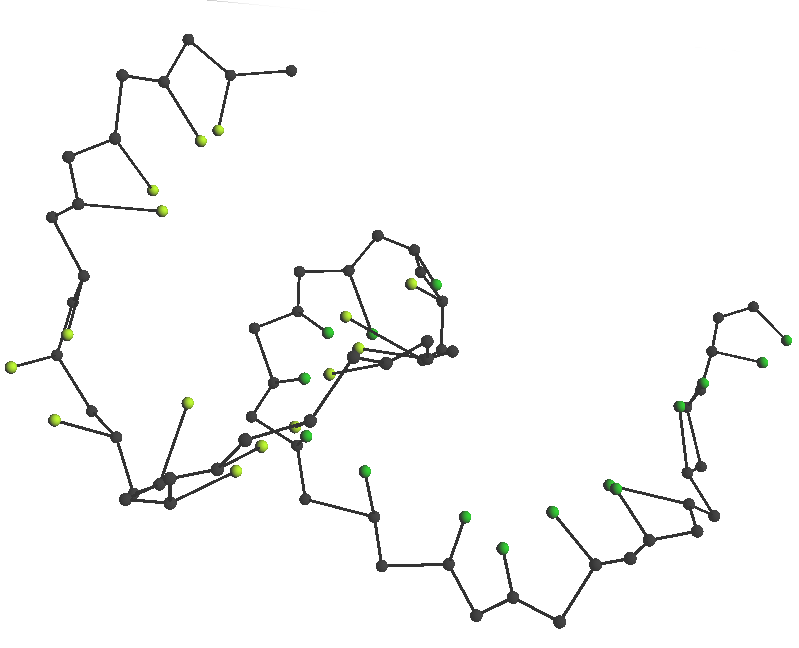
\includegraphics[width=4cm]{images/G15C15_1}
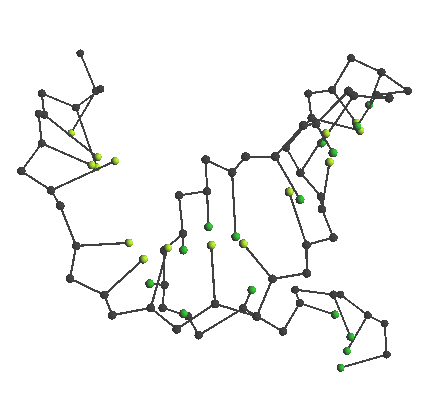
\includegraphics[width=4cm]{images/G15C15_2}
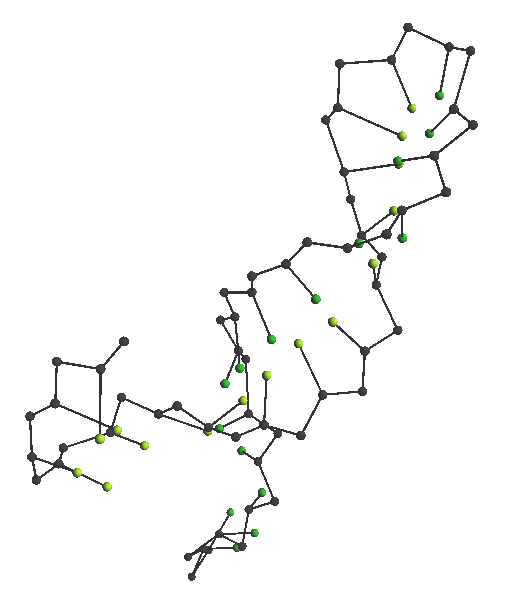
\includegraphics[width=4cm]{images/G15C15_3}
\end{center}
\caption{Visualisation of various stages of hairpin formation in a single strand of C$_{15}$G$_{15}$. In this case, the formation started at the center and zipped outwards.}
\label{results_hairpin}
\end{figure}


\input{images/hairpinScaling}







